\subsection*{(a)}
\subsubsection*{1.}
\FloatBarrier
\Cref{defaults_parallel} shows the default options. We run this on a Laptop with 8 parallel processes and we see that the default options change compared to sequential case. Now the default uses block jacobi, which was not the case when running with one process only.
\begin{table}[h!]
\centering
\begin{tabular}{ll}
\hline
\textbf{Option} & \textbf{Value} \\
\hline
KSP Type & gmres \\
Restart Size & 30 \\
Orthogonalization & Classical Gram-Schmidt \\
Tolerance & $10^{-5}$ (relative), $10^{-50}$ (absolute) \\
PC Type & bjacobi \\
Number of Blocks & 8 \\
Sub-PC Type & ilu (0 levels of fill) \\
Matrix Type & mpiaij \\
\hline
\end{tabular}
\caption{Default KSP and PC options}
\label{defaults_parallel}
\end{table}




\FloatBarrier


\subsubsection*{2.}
\FloatBarrier
The default Krylov and preconditioner combination as seen in the previous part is not recommendable for our problem in particular. Both, gmres and ilu are univerisal and make no use of the symmetric structure. However, we see in \Cref{nomgcombos}, it is still much better than not applying any preconditioning at all. We also see in \Cref{nomgcombos} that CG works much better, which makes sense because it is specifically designed for symmetric positive definite matrices.







\FloatBarrier


\subsubsection*{3.}
\FloatBarrier
We record the required quantities in \Cref{nomgcombos}. We see that compared to our base model, these models can use at least an order higher number of FLOPS/sec due to parallel execution.
\\
For GMRES with and without preconditioning, we read off the table that the execution time is in fact not proportional to the number of iterations. This might be due to high message passing activities which we also see in \Cref{nomgcombos}.
\\
We plot the curve of the residual of CG with and without preconditioning in \Cref{CG_plot}. Though not exactly, we see an overall monotonically decreasing trend. The small spikes in the not preconditioned CG can come from rounding errors that amplify strongly due to the large condition number of the matrix.
\\
Overall we see that preconditioning pays off in all cases. The direct solvers are about an order slower than the parallelizable algorithms, which was also to be expected.

\begin{table}[h!]
\hspace{-2.5cm}\begin{tabular}{lccccc}
\hline
\textbf{Method} & \textbf{KSP Iterations} & \textbf{Error} & \textbf{Wall Clock Time (s)} & \textbf{Flops/sec} & \textbf{MPI Msg Count} \\
\hline
GMRES no PC (30 vecs) & 10000 & 0.0099491 & 1.455e+01 & 2.895e+08 & 4.135e+04 \\
GMRES no PC (15 vecs) & 10000 & 0.0217839 & 1.470e+01 & 1.763e+08 & 4.268e+04 \\
GMRES no PC (60 vecs) & 10000 & 0.00241019 & 2.062e+01  & 3.634e+08 & 4.068e+04 \\
GMRES no PC (200 vecs) & 10000 & 5.24349e-06 & 4.335e+01 & 5.283e+08 & 4.021e+04 \\
\hline
GMRES Jacobi ILU (30 vecs) & 7225 & 1.17312e-06 & 2.705e+01  & 1.260e+08 & 2.988e+04 \\
GMRES Jacobi ILU (15 vecs) & 5881 & 1.16662e-06 & 3.188e+01  & 5.742e+07 & 2.511e+04 \\
GMRES Jacobi ILU (60 vecs) & 3943 & 1.17264e-06 & 2.040e+01 & 1.542e+08 & 1.605e+04 \\
GMRES Jacobi ILU (200 vecs) & 1723 & 1.07208e-06 & 1.346e+01 & 2.918e+08 & 6.940e+03 \\
\hline
CG without PC & 2048 & 0.000399514 & 6.701e+00 &  3.458e+05 & 6.156e+03 \\
CG with Jacobi & 373 & 0.00039954 & 7.011e+00 &  8.329e+04 & 1.131e+03 \\
\hline
LU Direct Solver & 1 & 4.81122e-08  & 4.956e+01 & 4.745e+08 & 0 \\
Cholesky (ND) & 1 & 4.81122e-08 & 1.414e+02 & 1.107e+06  & 0 \\
Cholesky (RCM) & 1 & 4.81122e-08 & 1.515e+02 & 1.033e+06 & 0 \\
\hline
\end{tabular}
\caption{Poisson Solver Results}
\label{nomgcombos}
\end{table}

\begin{figure}[h!]
\centering
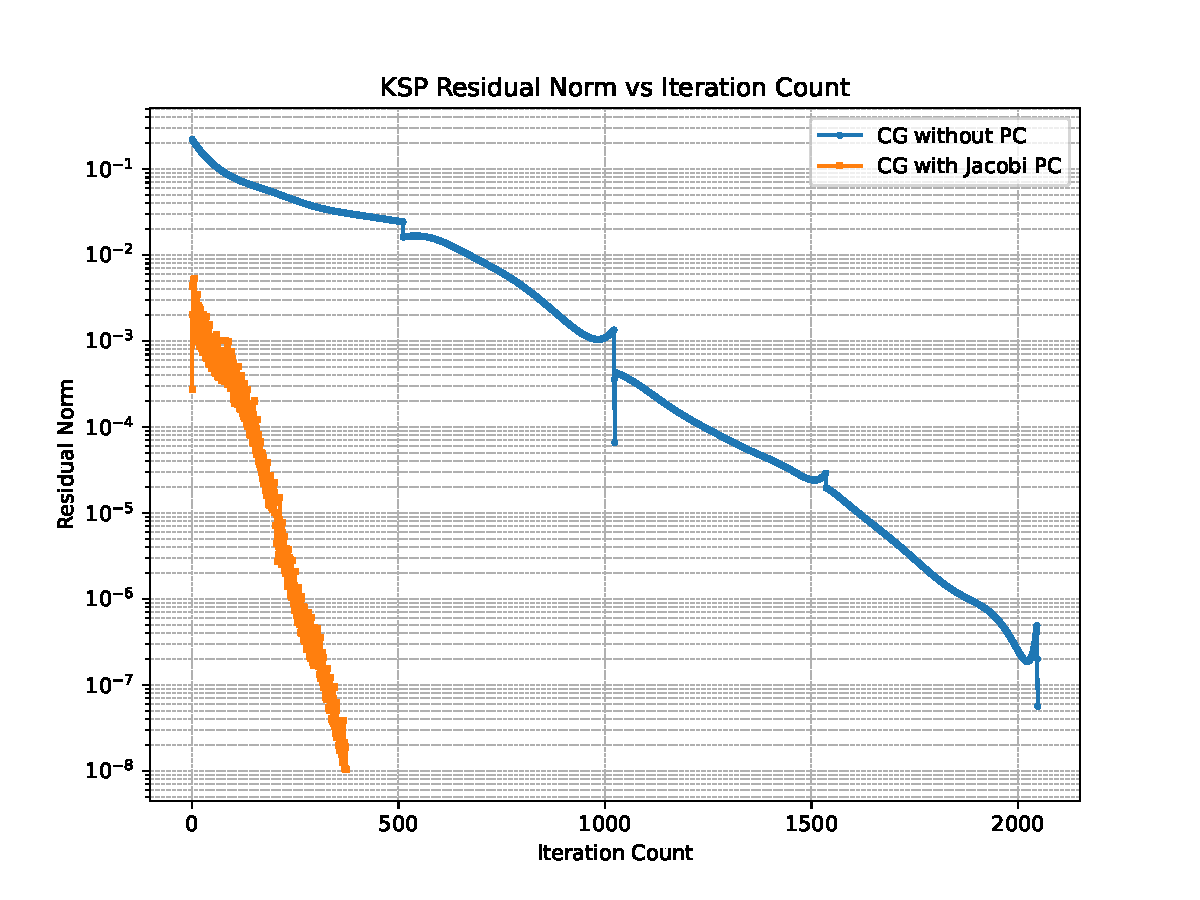
\includegraphics[width=0.85\textwidth]{CGplot.pdf}
\caption{Redidual curves of CG with and without PC}
\label{CG_plot}
\end{figure}
\FloatBarrier


\subsubsection*{4.}
\FloatBarrier
We record the results of our simulations in \Cref{tab:ex5.4} and observe that the Jacobi-preconditioned needs significantly fewer iterations with growing resolution. This is because the CG method depends strongly on the condition number of the system and (Jacobi-)preconditioning helps to deal with high condition numbers. The ICC can give further lower iteration counts for our problem because it makes use of the symmetric structure. Jacobi preconditioning does not do that.

\begin{table}[h!]
\hspace{-2.5cm}\begin{tabular}{lccccc}
\hline
\textbf{Method} & \textbf{KSP Iterations} & \textbf{Error} & \textbf{Wall Clock Time (s)} & \textbf{Flops/sec} & \textbf{MPI Msg Count} \\
\hline
CG no PC (0 refine) & 17 & 0.00076388 & 1.313e+00 & 3.931e+03 & 6.300e+01  \\
CG no PC (2 refine) & 73 & 4.91819e-05 & 6.171e-01 & 1.088e+05 & 3.080e+02  \\
CG no PC (4 refine) & 299 & 3.07512e-06 & 1.452e+00  & 6.516e+05 & 1.212e+03 \\
CG no PC (6 refine) & 1227 & 1.94253e-07 & 4.377e+00 & 3.276e+06 & 4.924e+03 \\
\hline
CG with Jacobi PC (0 refine) & 13 & 0.000763991 & 7.761e-01 & 7.003e+03  & 5.100e+01  \\
CG with Jacobi PC (2 refine) & 41 & 4.91809e-05 & 5.552e-01 & 9.475e+04 & 1.800e+02  \\
CG with Jacobi PC (4 refine) & 129 & 3.07288e-06 & 1.868e+00  &2.934e+05  & 5.080e+023 \\
CG with Jacobi PC (6 refine) & 450 & 1.98955e-07 & 4.506e+00 & 1.654e+06 & 1.816e+03 \\
\hline
\end{tabular}
\caption{Poisson Solver Results CG Refinements}
\label{tab:ex5.4}
\end{table}

\FloatBarrier



\subsubsection*{5.}
\FloatBarrier
We record the data on the multigrid methods to \Cref{mgcombos}. One can clearly see that these are in terms of the wall clock time much faster than most of the other methods. Moreover, Hypre's BoomerAMG has on top a surprisingly small message count.

\begin{table}[h!]
\hspace{-2.5cm}\begin{tabular}{lccccc}
\hline
\textbf{Method} & \textbf{KSP Iterations} & \textbf{Error} & \textbf{Wall Clock Time (s)} & \textbf{Flops/sec} & \textbf{MPI Msg Count} \\
\hline
PCGAMG 2 levels & 7 & 7.1221e-07 & 5.842e+00 & 1.433e+06 & 3.198e+03  \\
PCGAMG 4 levels & 7 & 7.1221e-07 & 6.522e+00 & 1.283e+06 & 3.198e+03  \\
PCGAMG 12 levels & 7 & 7.1221e-07 & 6.412e+00  & 1.306e+06 & 3.198e+03 \\
\makecell{PCGAMG 3 levels, \\ 3 choices for KSP, PC}& 7 & 1.94253e-07 & 4.407e+00 & 2.022e+06 & 3.340e+03 \\
\hline
W-cycle multigrid & 7 & 0.00205431 & 3.941e+00 & 3.065e+06  &3.646e+03  \\
CG with Jacobi PC (2 refine) & 41 & 4.91809e-05 & 5.552e-01 & 9.475e+04 & 1.800e+02  \\
MG type additive & 20 & 0.00638369 & 4.586e+00  &3.988e+06  & 4.454e+03 \\
MG type full & 4 & 8.96908e-05 & 5.474e+00 & 2.101e+06 & 5.722e+03 \\
MG Galerkin Process & 7 & 0.00161951 & 5.351e+00 & 2.341e+06 & 3.212e+03 \\
Hypre BoomerAMG & 4 & 1.16158e-06 & 3.716e+00 & 1.572e+05 & 3.200e+01 \\
\hline
\end{tabular}
\caption{Poisson Solver Results CG Refinements}
\label{mgcombos}
\end{table}
\FloatBarrier

\subsection*{(b)}
\FloatBarrier
In \Cref{3Dtable} we record the KSP convergence for CG + Block Jacobi and CG + BoomerAMG. We observe that the multigrid variant needs much less iterations at the 3rd and 4th refinement. However, The average runtimes are slightly slower with BoomerAMG. Unfortunately, we receive an error when refining further and attempting to solve this with BoomerAMG:
\\

\texttt{
srun: job 3684994 queued and waiting for resources\\
srun: job 3684994 has been allocated resources\\
xpmem\_attach error: : No such file or directory\\
srun: error: nid00163: task 220: Killed\\
srun: Terminating StepId=3684994.
}

\begin{table}[h!]
\centering
\begin{tabular}{|l|l|l|}
\hline
 & \text{KSP iterations} & Average Runtime\\ \hline
 CG + Block Jacobi + ICC (refine 3) & 155 & 2.305e+00 \\ \hline
 CG + Block Jacobi + ICC (refine 4) & 270 & 4.397e+00 \\ \hline
  CG + Block Jacobi + ICC (refine 5) & 536 & 1.635e+01 \\ \hline
   CG + Block Jacobi + ICC (refine 6) & 1082 & 1.178e+02\\ \hline
CG +  BoomerAMG (refine 3) & 5 & 3.316e+01\\ \hline
CG +  BoomerAMG (refine 4) & 4 &  1.917e+01\\ \hline
\end{tabular}
\caption{KSP iterations in 3D}
\label{3Dtable}
\end{table}


\FloatBarrier





